\let\negmedspace\undefined
\let\negthickspace\undefined
\documentclass[journal]{IEEEtran}
\usepackage[a5paper, margin=10mm, onecolumn]{geometry}
%\usepackage{lmodern} % Ensure lmodern is loaded for pdflatex
\usepackage{tfrupee} % Include tfrupee package

\setlength{\headheight}{1cm} % Set the height of the header box
\setlength{\headsep}{0mm}     % Set the distance between the header box and the top of the text

\usepackage{gvv-book}
\usepackage{gvv}
\usepackage{cite}
\usepackage{amsmath,amssymb,amsfonts,amsthm}
\usepackage{algorithmic}
\usepackage{graphicx}
\usepackage{textcomp}
\usepackage{xcolor}
\usepackage{txfonts}
\usepackage{listings}
\usepackage{enumitem}
\usepackage{mathtools}
\usepackage{gensymb}
\usepackage{comment}
\usepackage[breaklinks=true]{hyperref}
\usepackage{tkz-euclide} 
\usepackage{listings}
% \usepackage{gvv}                                        
\def\inputGnumericTable{}                                 
\usepackage[latin1]{inputenc}                                
\usepackage{color}                                            
\usepackage{array}                                            
\usepackage{longtable}                                       
\usepackage{calc}                                             
\usepackage{multirow}                                         
\usepackage{hhline}                                           
\usepackage{ifthen}                                           
\usepackage{lscape}
\begin{document}

\bibliographystyle{IEEEtran}
\vspace{3cm}

\title{9.2.27}
\author{EE25BTECH11060 - V.Namaswi}
% \maketitle
% \newpage
% \bigskip
{\let\newpage\relax\maketitle}
\renewcommand{\thefigure}{\theenumi}
\renewcommand{\thetable}{\theenumi}
\setlength{\intextsep}{10pt} % Space between text and floats
\textbf{Question}\\Find the Area enclosed by the parabola $4y=3x^2$ and the Line 2y=3x+12\\
\textbf{Solution}\\
Given Line 
\begin{align}
2y=3x+12\\
\vec{x}=\vec{h}+k\vec{m} ; k \in \mathbb{R}\\
\vec{h} = \begin{pmatrix} 0 \\ 6 \end{pmatrix}\\ \quad 
\vec{m} = \begin{pmatrix} 2 \\ 3 \end{pmatrix}
\end{align}
Given curve
\begin{align}
    4y=3 x^2\\
    \vec{x}^\top \vec{V} \vec{x} + 2\vec{u}^\top \vec{x} + f = 0\\
    \vec{V} = \begin{pmatrix} 3 & 0 \\ 0 & 0 \end{pmatrix}\\ \quad
\vec{u} = \begin{pmatrix} 0 \\ -2 \end{pmatrix} \\ \quad
f = 0
\end{align}
Points of Intersection\\
\begin{align}
    \kappa_i = \frac{1}{\vec{m}^\top \vec{V} \vec{m}} 
\left( -\vec{m}^\top (\vec{V}\vec{h} + \vec{u}) 
\pm \sqrt{ \left[ \vec{m}^\top (\vec{V}\vec{h} + \vec{u}) \right]^2 
- g(\vec{h}) \cdot (\vec{m}^\top \vec{V} \vec{m}) } \right)
\end{align}
where
\begin{align}
    g(\vec{h}) = \vec{h}^\top \vec{V} \vec{h} 
+ 2\vec{u}^\top \vec{h} + f\\
\vec{V}\vec{h} &= \begin{pmatrix} 3 & 0 \\ 0 & 0 \end{pmatrix}
\begin{pmatrix} 0 \\ 6 \end{pmatrix} = \begin{pmatrix} 0 \\ 0 \end{pmatrix} \\
\vec{V}\vec{h} + \vec{u} &= \begin{pmatrix} 0 \\ -2 \end{pmatrix} \\
\vec{m}^\top (\vec{V}\vec{h} + \vec{u}) &= 
\begin{pmatrix} 2 & 3 \end{pmatrix} \begin{pmatrix} 0 \\ -2 \end{pmatrix} 
= -6 \\
\vec{m}^\top \vec{V} \vec{m} &= 
\begin{pmatrix} 2 & 3 \end{pmatrix} 
\begin{pmatrix} 3 & 0 \\ 0 & 0 \end{pmatrix} 
\begin{pmatrix} 2 \\ 3 \end{pmatrix} = 
\begin{pmatrix} 2 & 3 \end{pmatrix} \begin{pmatrix} 6 \\ 0 \end{pmatrix} = 12 \\
\vec{u}^\top \vec{h} &= 
\begin{pmatrix} 0 & -2 \end{pmatrix} \begin{pmatrix} 0 \\ 6 \end{pmatrix} = -12 \\
g(\vec{h}) &= 0 + 2(-12) + 0 = -24\\
\kappa_i &= \frac{1}{12} \left(6 \pm \sqrt{(-6)^2 - (-24)(12)}\right) \\
&= \frac{1}{12} \left(6 \pm \sqrt{36 + 288}\right) \\
&= \frac{1}{12} \left(6 \pm \sqrt{324}\right)\\ 
=\frac{1}{12} (6 \pm 18)\\
= \kappa_1 = \frac{24}{12} = 2, \quad 
\kappa_2 = \frac{-12}{12} = -1
\end{align}
The point of intersection are :
\begin{align}
    (4, 12) \quad \text{and} \quad (-2, 3)
\end{align}
Area Bounded by curves is given by \\
\begin{align}
   \left | \int_{-2}^{4} \frac{3x^2}{4}-\frac{3x+12}{2} \right |\\
   = \left |\frac{1}{4}\int_{-2}^{4} 3 x^2 -6x -24  \right |\\
   = \left |\frac{1}{4}\brak{ x^3 -3 x^2 -24 x }_{-2}^{4} \right |\\
   =\left | \frac{1}{4}\brak{4^3 - (-2)^3 -3(4^2 - (-2)^2) -24(4-(-2)} \right |\\
           =27 
\end{align}
\begin{align}
\centering
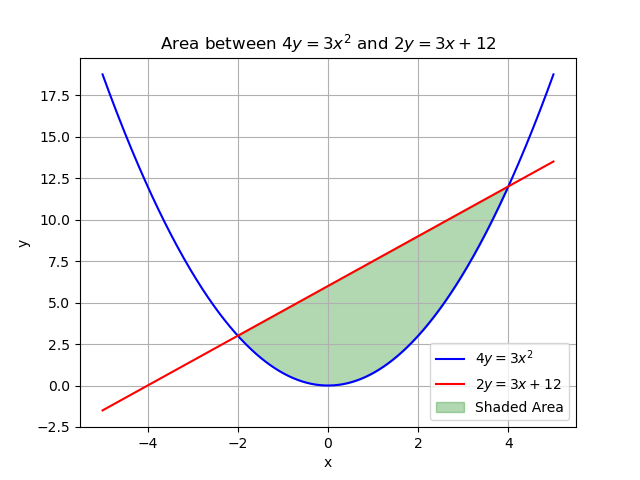
\includegraphics[width=\columnwidth, height=0.8\textheight, keepaspectratio]{figs/Figure_15.png}       
\end{align}
\end{document}
